\documentclass{standalone}
\usepackage{tikz}
\usetikzlibrary{patterns, positioning}


\begin{document}
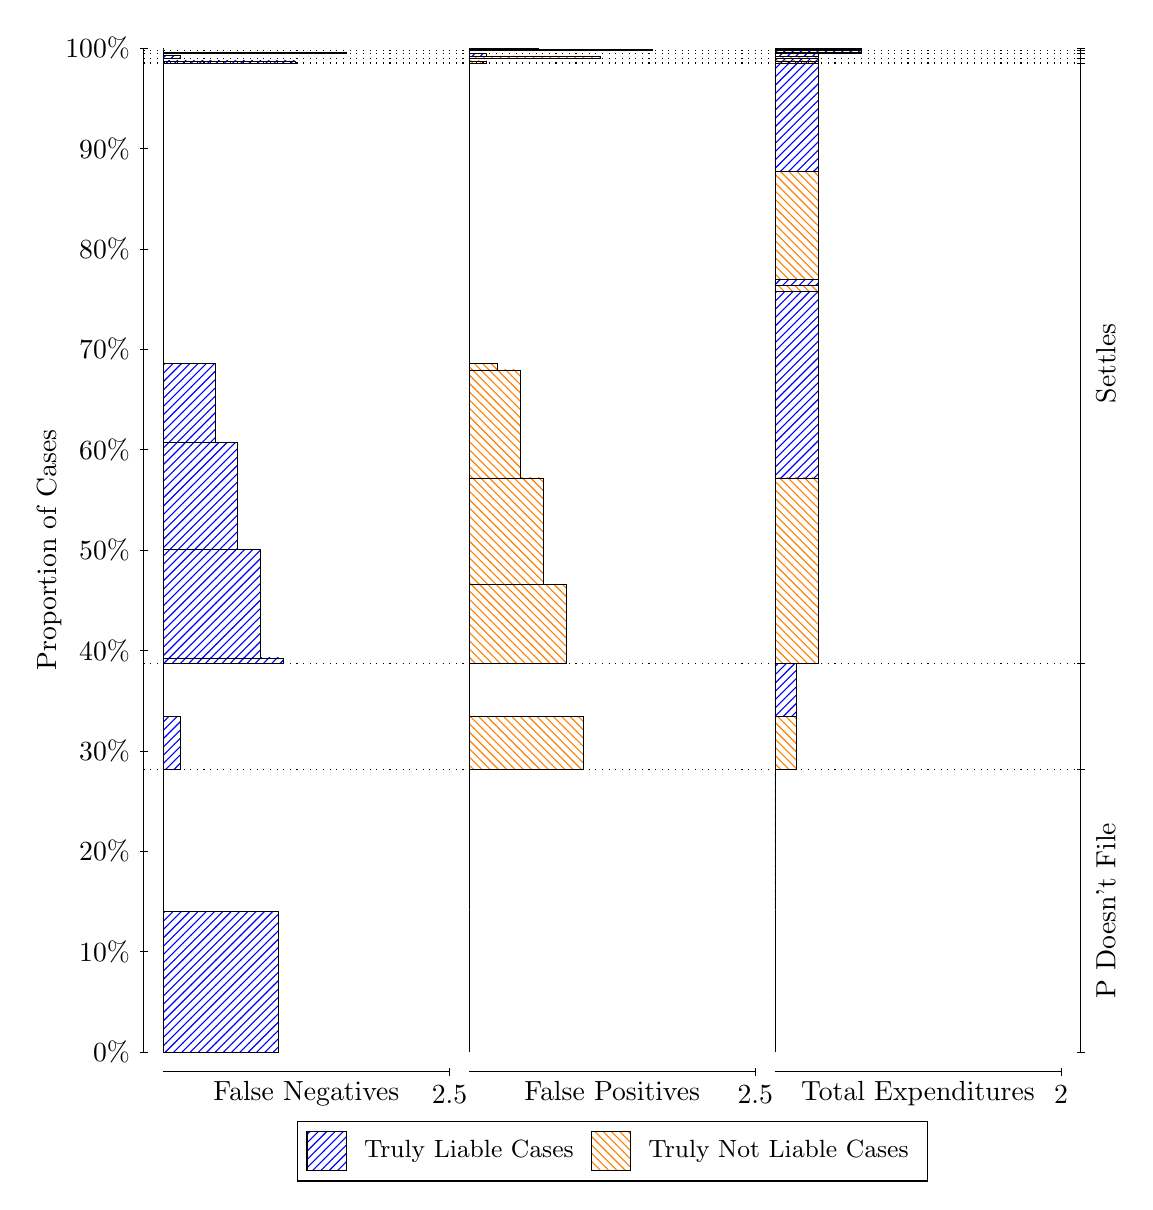
\begin{tikzpicture}
\draw[black, very thin] (1.5,1.75) -- (1.5,14.5);
\node[rotate=90, text=black, anchor=center] at (0.3, 8.125) {Proportion of Cases};
\draw[black, very thin] (1.45,1.75) -- (1.55,1.75);
\node[text=black, anchor=east] at (1.45, 1.75) {0\%};
\draw[black, very thin] (1.45,3.025) -- (1.55,3.025);
\node[text=black, anchor=east] at (1.45, 3.025) {10\%};
\draw[black, very thin] (1.45,4.3) -- (1.55,4.3);
\node[text=black, anchor=east] at (1.45, 4.3) {20\%};
\draw[black, very thin] (1.45,5.575) -- (1.55,5.575);
\node[text=black, anchor=east] at (1.45, 5.575) {30\%};
\draw[black, very thin] (1.45,6.85) -- (1.55,6.85);
\node[text=black, anchor=east] at (1.45, 6.85) {40\%};
\draw[black, very thin] (1.45,8.125) -- (1.55,8.125);
\node[text=black, anchor=east] at (1.45, 8.125) {50\%};
\draw[black, very thin] (1.45,9.4) -- (1.55,9.4);
\node[text=black, anchor=east] at (1.45, 9.4) {60\%};
\draw[black, very thin] (1.45,10.675) -- (1.55,10.675);
\node[text=black, anchor=east] at (1.45, 10.675) {70\%};
\draw[black, very thin] (1.45,11.95) -- (1.55,11.95);
\node[text=black, anchor=east] at (1.45, 11.95) {80\%};
\draw[black, very thin] (1.45,13.225) -- (1.55,13.225);
\node[text=black, anchor=east] at (1.45, 13.225) {90\%};
\draw[black, very thin] (1.45,14.5) -- (1.55,14.5);
\node[text=black, anchor=east] at (1.45, 14.5) {100\%};

\draw[black, very thin] (13.4,1.75) -- (13.4,14.5);
\draw[black, very thin] (13.35,1.75) -- (13.45,1.75);
\node[anchor=west] at (13.35, 1.75) {};
\draw[black, very thin] (13.35,5.3391) -- (13.45,5.3391);
\node[anchor=west] at (13.35, 5.3391) {};
\draw[black, very thin] (13.35,6.6812) -- (13.45,6.6812);
\node[anchor=west] at (13.35, 6.6812) {};
\draw[black, very thin] (13.35,14.31) -- (13.45,14.31);
\node[anchor=west] at (13.35, 14.31) {};
\draw[black, very thin] (13.35,14.365) -- (13.45,14.365);
\node[anchor=west] at (13.35, 14.365) {};
\draw[black, very thin] (13.35,14.433) -- (13.45,14.433);
\node[anchor=west] at (13.35, 14.433) {};
\draw[black, very thin] (13.35,14.466) -- (13.45,14.466);
\node[anchor=west] at (13.35, 14.466) {};
\draw[black, very thin] (13.35,14.5) -- (13.45,14.5);
\node[anchor=west] at (13.35, 14.5) {};

\draw[black, very thin, pattern color=blue, pattern=north east lines] (1.75,1.75) rectangle (3.2033,3.5325);
\draw[black, very thin, pattern color=orange, pattern=north west lines] (1.75,3.5325) rectangle (1.75,5.3391);
\draw[black, very thin, pattern color=blue, pattern=north east lines] (1.75,5.3391) rectangle (1.968,6.0102);
\draw[black, very thin, pattern color=orange, pattern=north west lines] (1.75,6.0102) rectangle (1.75,6.6812);
\draw[black, very thin, pattern color=blue, pattern=north east lines] (1.75,6.6812) rectangle (3.276,6.7562);
\draw[black, very thin, pattern color=blue, pattern=north east lines] (1.75,6.7562) rectangle (2.9853,8.1344);
\draw[black, very thin, pattern color=blue, pattern=north east lines] (1.75,8.1344) rectangle (2.6947,9.492);
\draw[black, very thin, pattern color=blue, pattern=north east lines] (1.75,9.492) rectangle (2.404,10.499);
\draw[black, very thin, pattern color=orange, pattern=north west lines] (1.75,10.499) rectangle (1.75,14.31);
\draw[black, very thin, pattern color=blue, pattern=north east lines] (1.75,14.31) rectangle (3.4213,14.338);
\draw[black, very thin, pattern color=orange, pattern=north west lines] (1.75,14.338) rectangle (1.75,14.365);
\draw[black, very thin, pattern color=blue, pattern=north east lines] (1.75,14.365) rectangle (1.968,14.406);
\draw[black, very thin, pattern color=orange, pattern=north west lines] (1.75,14.406) rectangle (1.75,14.433);
\draw[black, very thin, pattern color=blue, pattern=north east lines] (1.75,14.433) rectangle (4.0753,14.449);
\draw[black, very thin, pattern color=orange, pattern=north west lines] (1.75,14.449) rectangle (1.75,14.466);
\draw[black, very thin, pattern color=orange, pattern=north west lines] (1.75,14.466) rectangle (1.75,14.481);
\draw[black, very thin, pattern color=blue, pattern=north east lines] (1.75,14.481) rectangle (1.75,14.5);
\draw[black, very thin, pattern color=orange, pattern=north west lines] (5.6333,1.75) rectangle (5.6333,3.5566);
\draw[black, very thin, pattern color=blue, pattern=north east lines] (5.6333,3.5566) rectangle (5.6333,5.3391);
\draw[black, very thin, pattern color=orange, pattern=north west lines] (5.6333,5.3391) rectangle (7.0867,6.0102);
\draw[black, very thin, pattern color=blue, pattern=north east lines] (5.6333,6.0102) rectangle (5.6333,6.6812);
\draw[black, very thin, pattern color=orange, pattern=north west lines] (5.6333,6.6812) rectangle (6.8687,7.6878);
\draw[black, very thin, pattern color=orange, pattern=north west lines] (5.6333,7.6878) rectangle (6.578,9.0408);
\draw[black, very thin, pattern color=orange, pattern=north west lines] (5.6333,9.0408) rectangle (6.2873,10.412);
\draw[black, very thin, pattern color=orange, pattern=north west lines] (5.6333,10.412) rectangle (5.9967,10.493);
\draw[black, very thin, pattern color=blue, pattern=north east lines] (5.6333,10.493) rectangle (5.6333,14.31);
\draw[black, very thin, pattern color=orange, pattern=north west lines] (5.6333,14.31) rectangle (5.8513,14.337);
\draw[black, very thin, pattern color=blue, pattern=north east lines] (5.6333,14.337) rectangle (5.6333,14.365);
\draw[black, very thin, pattern color=orange, pattern=north west lines] (5.6333,14.365) rectangle (7.3047,14.392);
\draw[black, very thin, pattern color=blue, pattern=north east lines] (5.6333,14.392) rectangle (5.8513,14.433);
\draw[black, very thin, pattern color=orange, pattern=north west lines] (5.6333,14.433) rectangle (5.6333,14.45);
\draw[black, very thin, pattern color=blue, pattern=north east lines] (5.6333,14.45) rectangle (5.6333,14.466);
\draw[black, very thin, pattern color=orange, pattern=north west lines] (5.6333,14.466) rectangle (7.9587,14.481);
\draw[black, very thin, pattern color=blue, pattern=north east lines] (5.6333,14.481) rectangle (6.5053,14.5);
\draw[black, very thin, pattern color=orange, pattern=north west lines] (9.5167,1.75) rectangle (9.5167,3.5566);
\draw[black, very thin, pattern color=blue, pattern=north east lines] (9.5167,3.5566) rectangle (9.5167,5.3391);
\draw[black, very thin, pattern color=orange, pattern=north west lines] (9.5167,5.3391) rectangle (9.7892,6.0102);
\draw[black, very thin, pattern color=blue, pattern=north east lines] (9.5167,6.0102) rectangle (9.7892,6.6812);
\draw[black, very thin, pattern color=orange, pattern=north west lines] (9.5167,6.6812) rectangle (10.062,9.0408);
\draw[black, very thin, pattern color=blue, pattern=north east lines] (9.5167,9.0408) rectangle (10.062,11.405);
\draw[black, very thin, pattern color=orange, pattern=north west lines] (9.5167,11.405) rectangle (10.062,11.486);
\draw[black, very thin, pattern color=blue, pattern=north east lines] (9.5167,11.486) rectangle (10.062,11.561);
\draw[black, very thin, pattern color=orange, pattern=north west lines] (9.5167,11.561) rectangle (10.062,12.932);
\draw[black, very thin, pattern color=blue, pattern=north east lines] (9.5167,12.932) rectangle (10.062,14.31);
\draw[black, very thin, pattern color=orange, pattern=north west lines] (9.5167,14.31) rectangle (10.062,14.337);
\draw[black, very thin, pattern color=blue, pattern=north east lines] (9.5167,14.337) rectangle (10.062,14.365);
\draw[black, very thin, pattern color=orange, pattern=north west lines] (9.5167,14.365) rectangle (10.062,14.392);
\draw[black, very thin, pattern color=blue, pattern=north east lines] (9.5167,14.392) rectangle (10.062,14.433);
\draw[black, very thin, pattern color=orange, pattern=north west lines] (9.5167,14.433) rectangle (10.607,14.45);
\draw[black, very thin, pattern color=blue, pattern=north east lines] (9.5167,14.45) rectangle (10.607,14.466);
\draw[black, very thin, pattern color=orange, pattern=north west lines] (9.5167,14.466) rectangle (10.607,14.481);
\draw[black, very thin, pattern color=blue, pattern=north east lines] (9.5167,14.481) rectangle (10.607,14.5);
\draw[black, dotted] (1.5,5.3391) -- (13.4,5.3391);
\draw[black, dotted] (1.5,6.6812) -- (13.4,6.6812);
\draw[black, dotted] (1.5,14.31) -- (13.4,14.31);
\draw[black, dotted] (1.5,14.365) -- (13.4,14.365);
\draw[black, dotted] (1.5,14.433) -- (13.4,14.433);
\draw[black, dotted] (1.5,14.466) -- (13.4,14.466);
\draw[black, very thin] (1.75,1.5) -- (5.3833,1.5);
\node[text=black, anchor=north] at (3.5667, 1.5) {False Negatives};
\draw[black, very thin] (5.3833,1.45) -- (5.3833,1.55);
\node[text=black, anchor=north] at (5.3833, 1.45) {2.5};

\draw[black, very thin] (5.6333,1.5) -- (9.2667,1.5);
\node[text=black, anchor=north] at (7.45, 1.5) {False Positives};
\draw[black, very thin] (9.2667,1.45) -- (9.2667,1.55);
\node[text=black, anchor=north] at (9.2667, 1.45) {2.5};

\draw[black, very thin] (9.5167,1.5) -- (13.15,1.5);
\node[text=black, anchor=north] at (11.333, 1.5) {Total Expenditures};
\draw[black, very thin] (13.15,1.45) -- (13.15,1.55);
\node[text=black, anchor=north] at (13.15, 1.45) {2};

\node[text=black, centered, rotate=90] at (13.72, 3.5446) {P Doesn't File};

\node[text=black, centered, rotate=90] at (13.72, 10.496) {Settles};





\draw (7.449999999999999,1.5) node[draw=none] (baseCoordinate) {};
\begin{scope}[align=center]
        \matrix[scale=0.5, draw=black, below=0.5cm of baseCoordinate, nodes={draw}, column sep=0.1cm]{
            \node[rectangle, draw, minimum width=0.5cm, minimum height=0.5cm, pattern color=blue, pattern=north east lines] {}; &
            \node[draw=none, font=\small, text=black] (B) {Truly Liable Cases}; &
            \node[rectangle, draw, minimum width=0.5cm, minimum height=0.5cm, pattern color=orange, pattern=north west lines] {}; &
            \node[draw=none, font=\small, text=black] (B) {Truly Not Liable Cases}; \\
            };
\end{scope}

\end{tikzpicture}
\end{document}